%!TEX root = /Users/louis/Documents/PhD/Deliverables/Thesis/thesis.tex

\chapter{Analysis}
The literature review presented in Chapter~\ref{LiteratureReview} motivated a deeper analysis of existing techniques for managing evolution in the context of MDE. Figure~\ref{fig:analysis_overview} summarises the objectives of this chapter. On the left are the artefacts used to produce those on the right. As shown in Figure~\ref{fig:analysis_overview}, examples of co-evolution were located (Section~\ref{sec:locating_data}) and used to analyse existing co-evolution techniques. Analysis led to a categorisation and comparison of existing co-evolution techniques (Section~\ref{sec:analysing_existing_techniques}) and to the identification of modelling framework characteristics that restrict the way in which co-evolution can be managed (Section~\ref{subsec:modelling_framework_characteristics}). Research requirements for this thesis were identified from the analysis presented in this chapter (Section~\ref{sec:requirements_identification}).


\begin{figure}[htbp]
  \begin{center}
    \leavevmode
    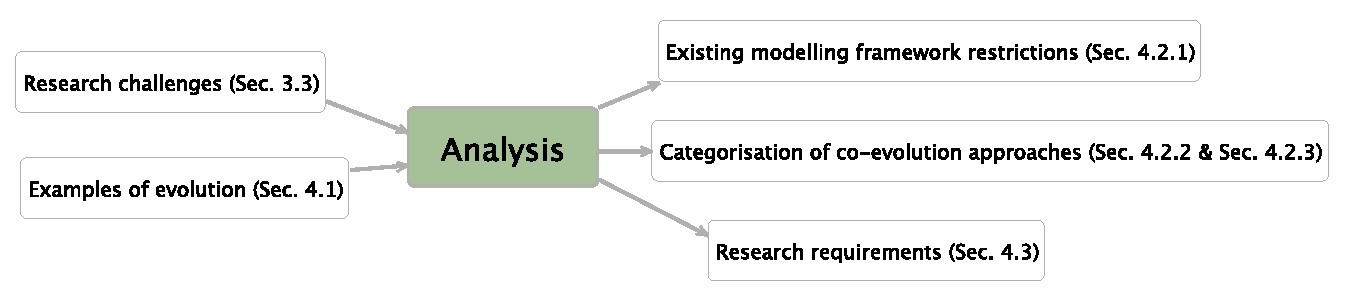
\includegraphics[scale=0.66]{4.Analysis/overview.pdf}
  \end{center}
  \caption{Analysis chapter overview.}
  \label{fig:analysis_overview}
\end{figure}


\section{Locating Data}
\label{sec:locating_data}
Two categories of evolutionary change encountered in model-driven engineering were identified in Chapter~\ref{Background}. Existing MDE projects were examined for examples of evolution, which would be used to provide requirements for developing structures and processes for evolutionary changes in the context of MDE. In this section, the requirements used to select example data are described, along with candidate and selected MDE projects. The section concludes with a discussion of further examples, which were obtained from collaborative research and from a related software engineering domain.  

\subsection{Requirements}
In Chapter~\ref{Background}, two categories of evolutionary change were identified: co-evolution and synchronisation. In this section, requirements are partitioned into three types: those necessary for studying each of the two categories of evolutionary change, and common requirements (applicable to both categories of evolutionary change).

\subsubsection{Common requirements}
Every candidate project needs to use MDE. Specifically, both metamodelling and model transformation must be used (requirement R1). In addition, each candidate project needs to provide historical information to trace the evolution of development artefacts (R2). For example, several versions of the project are needed perhaps in a source code management system. Finally, a candidate project needs to have undergone a number of significant changes\footnote{This is deliberately vague. Further details are given in Section~\ref{subsec:project_selection}.} (R3).

\subsubsection{Co-evolution requirements}
A candidate project for the study of co-evolution needs to define a metamodel and some changes to that metamodel (R4). In the projects considered, the metamodel changes took the form of either another version of the metamodel, or a history (which recorded each of the steps used to produce the adapted metamodel). A candidate project also needs to provide example instances of models before and after each migration activity (R5).

Ideally, a candidate project should include more than one consecutive metamodel adaptation, so as to represent the way in which the same development artefacts continue to evolve over time (optional requirement O1).

\subsubsection{Synchronisation requirements}
A candidate project for the study of synchronisation needs to define a model-to-model transformation (R6). Furthermore, a candidate project has to include many examples of source and target models for that transformation (R7). Crucially, a candidate project needs to provide many examples of the kinds of change (to either source or target model) that cause inconsistency between the models (R8). 

Ideally, a candidate project should also include transformation chains (more than one model-to-model transformation, executed sequentially) (O2). Chains of transformations are prescribed by the MDA guidelines \cite{kleppe03mda}.


\subsection{Project Selection}
\label{subsec:project_selection}
Eight candidates were considered for the study. Table \ref{tab:candidates} shows which of the requirements are fulfilled by each of the candidates. Each candidate is now discussed in turn.

\begin{table}
	\caption{Candidates for study of evolution in existing MDE projects}
	\centering
	\begin{tabular}{|c||c|c|c||c|c|c||c|c|c|c|}
		\hline
		\multirow{3}{*}{Name} & \multicolumn{10}{|c|}{Requirements} \\
		\cline{2-11}
		          & \multicolumn{3}{|c||}{Common} & \multicolumn{3}{|c||}{Co-evolution} & \multicolumn{4}{|c|}{Synchronisation} \\
		\cline{2-11}
		          & R1 & R2 & R3 & R4 & R5 & O1 & R6 & R7 & R8 & O2 \\
		\hline
		GSN       & x  &    &    & x  &    &    &    &    &    &    \\
		\hline
		OMG       & x  &    &    & x  &    &    & x  &    &    &    \\
		\hline
		Zoos      & x  & x  &    & x  &    &    &    &    &    &    \\
		\hline
		MDT       & x  & x  &    & x  &    & x  &    &    &    &    \\
		\hline
		MODELPLEX & x  & x  & x  & x  &    & x  & x  & x  &    &    \\
		\hline
		FPTC      & x  & x  & x  & x  & x  &    &    &    &    &    \\
		\hline
		xText     & x  & x  & x  & x  & x  & x  & x  & x  &    & x  \\
		\hline
		GMF       & x  & x  & x  & x  & x  & x  & x  & x  &    & x  \\
		\hline
	\end{tabular}
	\label{tab:candidates}
\end{table}

\subsubsection{GSN}
\label{par:gsn}
Georgios Despotou and Tim Kelly, members of this department's High Integrity Systems Engineering group, are constructing a metamodel for Goal Structuring Notation (GSN). The metamodel has been developed incrementally. There is no accurate and detailed version history for the GSN metamodel (requirement R2). \textbf{Suitability for study:} Unsuitable.

\subsubsection{OMG}
\label{par:omg}
The Object Management Group (OMG) \cite{omg} oversees the development of model-driven technologies. The Vice President and Technical Director of OMG, Andrew Watson, references the development of two MDE projects in \cite{watson08mdahistory}. Correspondence with Watson ascertained that source code is available for one of the projects, but there is no version history. \textbf{Suitability for study:} Unsuitable.

\subsubsection{Zoos}
\label{par:zoos}
A zoo is a collection of metamodels, authored in a common metamodelling language. I considered two zoos, but neither contained any significant external metamodel changes. Those changes that were made involved only renaming of meta-classes (trivial to migrate) or additive changes (which do not affect consistency, and therefore require no migration). \textbf{Suitability for study:} Unsuitable.

\subsubsection{MDT}
The Eclipse Model Development Tools (MDT) \cite{mdt} provides implementations of industry-standard metamodels, such as UML2 \cite{uml212} and OCL \cite{ocl2}. Like the metamodel zoos, the version history for the MDT metamodels contained no significant changes. \textbf{Suitability for study:} Unsuitable.

\subsubsection{MODELPLEX}
Jendrik Johannes, a research assistant at TU Dresden, has made available work from the European project, MODELPLEX. Johannes's work involves transforming UML models to Tool Independent Performance Models (TIPM) for simulation. Although the TIPM metamodel and the UML-to-TIPM transformation have been changed significantly, no significant changes have been made to the models. \textbf{Suitability for study:} Unsuitable.

\subsubsection{FPTC}
Failure Propagation and Transformation Calculus (FPTC), developed by Malcolm Wallace in this department, provides a means for reasoning about the failure behaviour of complex systems. Before starting my doctorate, I worked with Richard Paige to develop an implementation of FPTC in Eclipse. The implementation includes an FPTC metamodel. Recent work with Philippa Conmy, a research assistant in the department, has identified a significant flaw in the implementation, leading to changes to the metamodel. These changes caused existing FPTC models to become inconsistent with the metamodel. Conmy has made available copies of FPTC models from before and after the changes. \textbf{Suitability for study:} Suitable for studying co-evolution. Unsuitable for studying synchronisation.

\subsubsection{xText}
xText is an openArchitectureWare (oAW) \cite{oaw} tool for generating parsers, metamodels and editors for performing text-to-model transformation. Internally, xText defines a metamodel, which has been changed significantly over the last two years. In several cases, changes have caused inconsistency with existing models. xText provides examples of use, which have been updated alongside the metamodel. \textbf{Suitability for study:} Suitable for studying co-evolution. Unsuitable for studying synchronisation.

\subsubsection{GMF}
The Graphical Modelling Framework (GMF) \cite{gronback06gmf} allows the definition of graphical concrete syntax for metamodels that have been defined in EMF. GMF prescribes a model-driven approach: Users of GMF define concrete syntax as a model, which is used to generate a graphical editor. In fact, five models are used together to define a single editor using GMF.

GMF defines the metamodels for graphical, tooling and mapping definition models; and for generator models. The metamodels have changed considerably during the development of GMF. Some changes have caused inconsistency with GMF models. Presently, migration is encoded in Java. Gronback has stated\footnote{Private communication, 2008.} that the migration code is being ported to QVT (a model-to-model transformation language) as the Java code is difficult to maintain.

GMF fulfils almost all of the requirements for the study. A large amount of the co-evolution data is available, including migration strategies. The GMF source code repository does not contain examples of the kinds of change that cause inconsistency between the models. However, GMF has a large number of users, and it may be possible to gather this information elsewhere. \textbf{Suitability for study:} Suitable for studying both categories of evolutionary change.

\subsubsection{Summary of selection}
The FPTC and xText projects were selected for a study of co-evolution. No appropriate projects were located for a study of synchronisation. The GMF project will not be studied immediately, but reserved for evaluation (Chapter~\ref{Evaluation}).


\subsection{Other examples}
Because only a small number of MDE projects fulfilled all of the requirements, additional data was collected from alternative sources. Firstly, examples were sought from a related domains, object-oriented systems. Secondly, examples were discovered during collaboration with colleagues on two projects, both of which involved developing a system using MDE.

\subsubsection{Examples of evolution from object-oriented systems}
In object-oriented programming, software is constructed by developing groups of related objects. Every object is an instance of (at least) one class. A class is a description of characteristics, which are shared by each of the class's instances (objects). A similar relationship exists between models and metamodels: metamodels comprises meta-classes, which describe the characteristics shared by each of the meta-class's instances (elements of a model). Together, model elements are used to describe one perspective (model) of a system. This similarity between object-oriented programming and metamodelling implied that the evolution of object-oriented systems may be similar to evolution occurring in MDE. 

\emph{Refactoring} is the process of improving the structure of existing code while maintaining its external behaviour. When used as a noun, a refactoring is one such improvement. As discussed in Chapter~\ref{LiteratureReview}, refactoring of object-oriented systems has been widely studied, perhaps must notably in \cite{fowler99refactoring}, which provides a catalogue of refactorings for object-oriented systems. For each refactoring, Fowler gives advice and instructions for its application.

To explore their relevance to MDE, the refactorings described in \cite{fowler99refactoring} were applied to metamodels. Some were found to be relevant to metamodels, and could potential occur during MDE. Many were found to be irrelevant, belonging to one of the following three categories:

\begin{enumerate}
	\item \textbf{Operational refactorings} focus on restructuring behaviour (method bodies). Most modern MDE modelling frameworks do not support the specification of behaviour in models.
	\item \textbf{Navigational refactorings} convert, for example, between bi-directional and uni-directional associations. These changes are non-breaking in EMF, which automatically provides values for the inverse of a reference when required.
	\item \textbf{Domain-specific refactorings} manage issues specific to object-oriented programming, such as casting, defensive return values, and assertions. These issues are not relevant to metamodelling.
\end{enumerate}

The object-oriented refactorings that can be applied to metamodels provide examples of metamodel evolution. When applied, some of these refactorings potentially cause inconsistency between a metamodel and its models. By using Fowler's description of each refactoring, a migration strategy for updating (co-evolving) inconsistent models was deduced. An example of this process is now presented.

Figure \ref{fig:refactoring} illustrates a refactoring that changes a reference object to a value object. Value objects are immutable, and cannot be shared (i.e. any two objects cannot refer to the same value object). By contrast, reference objects are mutable, and can be shared. Figure \ref{fig:refactoring} indicates that applying the refactoring restricts the multiplicity of the association (on the Order end) to 1 (implied by the composition); prior to the refactoring the multiplicity is many-valued.

\begin{figure}[htbp]
  \begin{center}
    \leavevmode
    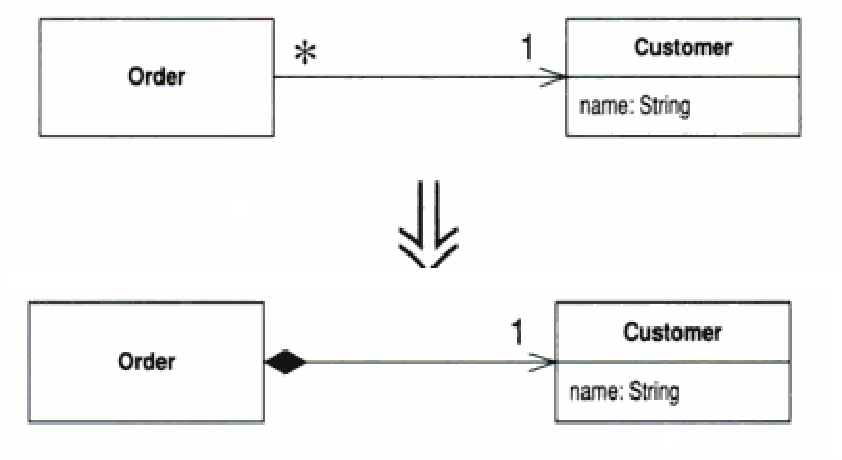
\includegraphics[scale=0.5]{4.Analysis/exemplar_refactoring.pdf}
  \end{center}
  \caption{Refactoring a reference to a value. Taken from \cite{fowler99refactoring}[pg183].}
  \label{fig:refactoring}
\end{figure}

Before applying the refactoring, each customer may be associated with more than one order. After the refactoring, each customer should be associated with only one order. Fowler indicates that every customer associated with more than one order should be duplicated, such that one customer object exists for each order. Therefore, the migration strategy in Listing \ref{lst:refactoring} is deduced. Using this process, migration strategies were deduced for each of the refactorings that were applicable to metamodelling, and caused inconsistencies between a metamodel and its models.

\begin{lstlisting}[caption=Migration strategy for the refactoring in pseudo code., label=lst:refactoring]
for every customer, c
  for every order, o, associated with c
    create a new customer, d
    copy the values of c's attributes into d
  next o
	
  delete c
next c
\end{lstlisting}

The examples of metamodel evolution based on Fowler's refactorings provided additional data for deriving research requirements. Some parts of the metamodel evolutions from existing MDE projects were later found to be equivalent to Fowler's refactorings, which, to some extent, validates the above claim that evolution from object-oriented systems can be used to reason about metamodel evolution.

On the other hand, object-oriented refactorings are used to improve the maintainability of existing systems. In other words, they represent only one of the three reasons for evolutionary change defined by \cite{sjoberg93quantifying}. The two other types of changes are equally relevant for deriving research requirements, and so object-oriented refactorings alone are not sufficient for reasoning about metamodel evolution.


\subsubsection{Research collaborations}
As well as the example data located from object-oriented system, collaboration on projects using MDE with two colleagues provided several examples of evolution. A prototypical metamodel to standardise the way in which process-oriented programs are modelled was produced with Adam Sampson, a research assistant at the University of Kent, and an investigation of the feasibility of implementing a tool for generating story-worlds for interactive narratives was conducted with Heather Barber, a postdoctorate student in the department.

In both cases, a metamodel was constructed for describing concepts in the domain. The metamodels were developed incrementally and changed over time. The collaborations with Sampson and Barber did not involve constructing model-to-model transformations, but did provide data suitable for a study of co-evolution.

Majority of the changes made in both of these projects related to changing requirements. In each iteration, existing requirements were refined and new requirements discovered. Neither project required changes to support architectural restructuring. In addition, the work undertaken with Sampson included some changes to adapt the system for use with a different technology than originally anticipated. That is to say, the changes observed represented two of the three reasons for evolutionary change defined by \cite{sjoberg93quantifying}. 


\subsection{Summary}
To summarise, in this section the example data used to analyse existing structures and processes for managing evolution in the context of MDE was discussed. Example data was sought from existing MDE projects, and also from a related domain and research collaboration. Eight existing MDE projects were located, three of which satisfied the requirements for a study of co-evolutionary changes in the context of model-driven engineering. One of the three projects, GMF, was reserved as a case study and is used for evaluation in Chapter~\ref{Evaluation}. Refactorings of object-oriented programming supplemented the data available from the existing MDE projects. Collaboration with Sampson and Barber yielded further examples of co-evolution.

Due to the lack of examples of model synchronisation, this thesis now focuses on model and metamodel co-evolution. 



\section{Analysing Existing Techniques}
\label{sec:analysing_existing_techniques}
% Having described the selection of suitable data for the analysis, we will then outline the way in which we have applied existing techniques to the data, and introduce criteria against which the effectiveness of existing techniques will be measured. 
The examples of co-evolution identified in the previous section were analysed to discover and compare existing techniques for managing co-evolution. This section discusses the results of analysing the examples; namely a deeper understanding of modelling framework characteristics that affect the management of co-evolution and a categorisation of existing techniques for managing co-evolution. These results were published in \cite{rose09analysis,rose09flock}.


\subsection{Modelling Framework Characteristics Relevant to Co-Evolution}
\label{subsec:modelling_framework_characteristics}
Analysis of the co-evolution examples identified in the previous section highlighted characteristics of modern MDE modelling development environments that impact on the way in which co-evolution can be managed.

Firstly, in modern MDE development environments, \emph{models and metamodels are separated}. Metamodels are developed and distributed to users. Metamodels are installed, configured and combined to form a customised MDE development environment. Metamodel developers have no programmatic access to downstream instance models. Consequently, metamodel evolution occurs independently to model migration. First, the metamodel is evolved. Subsequently, the users of the metamodel find that their models are out-of-date and migrate their models.

Because of model and metamodel separation, existing techniques for managing co-evolution are either \emph{developer-driven} (the metamodel developer devises an executable migration strategy, which is distributed to the metamodel user with the evolved metamodel) or \emph{user-driven} (the metamodel user devises the migration strategy). In either case, it is always the metamodel user who performs migration on models that no longer conform to the metamodel.

Secondly, modern MDE development environments \emph{implicitly enforce conformance}. A model is \emph{bound} to its metamodel, typically by constructing a representation in the underlying programming language for each model element and data value. Frequently, binding is strongly-typed: each metamodel type is mapped to a corresponding type in the underlying programming language using mappings defined by the metamodel. Consequently, MDE modelling frameworks do not permit changes to a model that would cause it to no longer conform to its metamodel. Loading a model that does not conforms to its metamodel causes an error. In short, MDE modelling frameworks cannot be used to manage any model that does not conform to its metamodel.

Consequently, user-driven migration is always a manual process, in which models are migrated without using the modelling framework (which is unable to load non-conformant models). Executable migration strategies can only be used if they are specified with a tool that does not depend on the modelling framework to load the non-conformant models (and, at present, no such tool exists). Typically then, the metamodel user can only perform migration by editing the model directly, normally manipulating its underlying representation (e.g. XMI).

Furthermore, model migration must produce a model that conforms to the evolved metamodel because MDE modelling frameworks do not permit changes to a model that cause non-conformance. Therefore, model migration cannot be specified as a combination of co-evolution techniques with each performing some part of the migration.

Finally, a further consequence of implicitly enforced conformance is that models cannot be checked for conformance against any metamodel other than their own. Because conformance is always assumed, modern MDE development environment provide limited mechanisms for checking conformance, and typically provide no support for checking conformance to a metamodel other than the one used to construct the model. As will be discussed in Chapter~\ref{Implementation}, conformance checking can be used during metamodel installation to highlight potential conformance problems, and to determine whether migration is necessary for a model, permitting improved scalability for automatic model migration techniques.


\subsection{User-Driven Co-Evolution}
Examples of co-evolution were analysed to discover and compare existing techniques for managing co-evolution. As discussed above, the separation of models and metamodels leads to two processes for co-evolution: \emph{developer-driven} and \emph{user-driven}. No existing research has explored user-driven co-evolution, yet several of the co-evolution examples identified in Section~\ref{sec:locating_data} employed a user-driven co-evolution approach. This section discusses user-driven co-evolution and describes a scenario (based on several of the co-evolution examples from Section~\ref{sec:locating_data}) to illustrate a user-driven co-evolution process.

In user-driven co-evolution, the metamodel user performs migration by locating non-conformant models and updating them to conform to the evolved metamodel. The metamodel developer might guide migration by providing a migration strategy to the metamodel user. Crucially, however, the migration strategy is not executable (e.g. it is written in prose). This is the key distinction between user-driven and developer-driven co-evolution. Only in the latter does the metamodel developer provided an executable model migration strategy.  

In some cases, the metamodel user will not be provided with any migration strategy (executable or otherwise) from the metamodel developer. To perform migration, the metamodel user must determine which (if any) model elements no longer conform to the evolved metamodel, and then decide how best to change non-conformant elements to re-establish conformance. This situation can be thought of as analogous to developing a legacy system\footnote{A system for which one has no documentation and whose authors have left the owning organisation.}.

\subsubsection{Scenario}
The following scenario demonstrates user-driven co-evolution. Mark is developing a metamodel using the Eclipse Modeling Framework (EMF). Members of his team, including Heather, will be using the metamodel to construct models. Heather installs the plug-in for Mark's metamodel and begins constructing models. Mark later identifies new requirements, changes the metamodel, builds a new version of the metamodel plug-in, and distributes it to Heather.

After several iterations of metamodel updates, Heather tries to load one of her older models, constructed using an earlier metamodel. When loading the older model, EMF reports an error indicating that the model no longer conforms to its metamodel. To load the older model, Heather must reinstall an old version of the metamodel plug-in that contains the metamodel to which the older model conforms. But even then, EMF will bind the older model to the old version of the metamodel, and not to the evolved metamodel. Worse still, Eclipse does not allow two versions of the same plug-in to co-exist in the same workspace, so the evolved metamodel cannot be used.

To avoid the loading errors in Heather's workspace, Mark could use an existing tool for managing co-evolution. However, all existing tools require extra effort from Mark (as discussed in Section~\ref{subsec:co-evolution_categorisation}).

Employing user-driven migration, Heather must trace and repair the loading error directly in XMI, the underlying format of the model. Human usability was not a key requirement for XMI \cite{hutn} and, consequently, using XMI for migration is an unproductive and tedious task. Worse still, as EMF only reports the first problem encountered when deserialising an inconsistent model, re-establishing consistency in XMI is a slow, iterative process.


\subsubsection{Challenges}
The above scenario highlights two of the major challenges faced when performing user-driven migration. Firstly, the underlying model representation is unlikely to be optimised for human usability. Together with limited support for conformance checking, user-driven migration performed by editing the underlying model representation is error prone and tedious. Secondly, installing a new version of a metamodel plug-in can affect the conformance of models and, moreover, conformance problems are not reported to the user as part of the installation process. These challenges are elaborated on further in the final section of this chapter, which identifies research requirements.


\subsection{Categorisation of Developer-Driven Co-Evolution Techniques}
\label{subsec:co-evolution_categorisation}
In developer-driven co-evolution, the metamodel developer provides an executable migration strategy along with the evolved metamodel. Model migration might be scheduled automatically (for example when a model is loaded) or by the metamodel user (when conformance problems for a model are reported).

Existing co-evolution research focuses on developer- rather than user-driven co-evolution. By applying existing co-evolution approaches to the co-evolution examples identified in Section X, existing developer-driven co-evolution approaches were categorised, compared and contrasted. Three categories of developer-driven co-evolution approach were identified, \emph{manual specification}, \emph{operator-based} and \emph{metamodel matching}. This categorisation was published in \cite{rose09analysis} and revisited in \cite{rose09flock}. Each category is now discussed.


\subsubsection{Manual Specification}
In \emph{manual specification}, the migration strategy is encoded manually by the metamodel developer, typically using a general purpose programming language (e.g. Java) or a model-to-model transformation language (such as QVT \cite{qvt}, or ATL \cite{jouault05transforming}). The migration strategy can manipulate instances of the metamodel in anyway permitted by the modelling framework and hence manual specification permits the metamodel developer the most control over model migration.

However, manual specification generally requires the most effort on the part of the metamodel developer for two reasons. Firstly, as well as implementing the migration strategy, the metamodel developer must also produce code for executing the migration strategy. Typically, this involves integration of the migration strategy with the modelling framework (to load and store models) and possibly with development tools (to provide a user interface). Secondly, frequently occurring model migration patterns -- such as copying a model element from original to migrated model -- are not captured by existing general purpose and model-to-model transformation languages, and so each metamodel developer has to devise his or her own abstractions.

\subsubsection{Operator-based Co-evolution}
\label{subsec:operator-based_co-evolution}
In \emph{operator-based co-evolution}, a library of \emph{co-evolutionary operators} is provided. Each co-evolutionary operator specifies a metamodel evolution along with a corresponding model migration strategy. For example, the ``Make Reference Containment'' operator evolves the metamodel such that a non-containment reference becomes a containment reference and migrates models such that the values of the evolved reference are replaced by copies. By composing co-evolutionary operators, metamodel evolution can be performed and a migration strategy can be generated without writing any code. Wachsmuth \cite{wachsmuth07metamodel} proposes a library of co-evolutionary operators for MOF metamodels. COPE \cite{herrmannsdoerfer09cope} is an operator-based co-evolution approach for the Eclipse Modeling Framework.

The usefulness of an operator-based co-evolution approach depends heavily on the richness of the library of co-evolutionary operators that it provides. When no appropriate co-evolutionary operator is available, the metamodel developer must use another approach for performing model migration. COPE allows metamodel developers to specify custom migration strategies when no co-evolutionary operator is appropriate, using a general purpose programming language. Consequently, custom migration strategies in COPE suffer one of the same limitations as manual specification approaches: model migration patterns are not captured in the language used to specify migration strategies. 

Therefore, it seems that operator-based co-evolution approaches should seek to provide a complete library of co-evolutionary operators, so that at least one operator is appropriate for every co-evolution that a metamodel developer may wish to perform. However, as discussed by Lerner \cite{lerner00model}, a large library of operators increases the complexity of specifying migration. To demonstrate, Lerner considers moving a feature from one type to another. This could be expressed by sequential application of two operators called, for example, \texttt{delete\_feature} and \texttt{add\_feature}. However, the semantics of a \texttt{delete\_feature} operator likely dictate that the  values of that feature will be removed during migration and hence, \texttt{delete\_feature} is unsuitable when specifying that a feature has been moved. To solve this problem, a \texttt{move\_feature} operator could be introduced, but then the metamodel developer must understand the difference between the two ways in which moving a type can be achieved, and carefully select the correct one. Lerner provides other examples which further elucidate this issue (such as introducing a new type by splitting an existing type). As the size of the library of co-evolutionary operators grows, so does the complexity of selecting appropriate operators and, hence, the complexity of performing metamodel evolution.

Clear communication of the effects of each co-evolutionary operator (on both the metamodel and its instance models) can improve the navigability of large libraries of co-evolutionary operators. COPE, for example, provides a name, description, list of parameters and applicability constraints for each co-evolutionary operator. An example, taken from\footnote{\url{http://cope.in.tum.de/pmwiki.php?n=Operations.MakeContainment}}, is shown below.

\begin{quote}
\textbf{Make Reference Containment}

In the metamodel, a reference is made containment. In the model, its values are replaced by copies.

\emph{Parameters}:
\begin{itemize}
	\item \texttt{reference}: The reference
\end{itemize}

\emph{Constraints}:
\begin{itemize}
	\item The \texttt{reference} must not already be containment.
\end{itemize}
\end{quote}

Other techniques can be used to try to improve the navigability of large libraries of co-evolutionary operators. For example, COPE restricts the choice of operators to only those that can be applied to the currently selected metamodel element. Finding a balance between a richness and navigability is a key challenge in defining libraries of co-evolutionary operators for operation-based co-evolution approaches. Analogously, a known challenge in the design of software interfaces is the trade-off between a rich and a concise interface \cite{bloch05apis}.

To perform metamodel evolution using co-evolutionary operators, the library of co-evolutionary operators must be integrated with tools for editing metamodels. COPE, for instance, provides integration with the EMF tree-based metamodel editor. However, some developers edit their metamodels using a textual syntax, such as Emfatic \cite{emfatic}. In general, freeform text editing is less restrictive than tree-based editing (because in the latter, the metamodel is always structurally sound whereas in the former, the text does not always have to compile). Consequently, it is not clear whether operator-based co-evolution can be used with all categories of metamodel editing tool.

\subsubsection{Metamodel Matching}
\label{subsec:metamodel_matching}
In \emph{metamodel matching}, a migration strategy is inferred by analysing the evolved metamodel and the \emph{metamodel history}. Metamodel matching approaches use one of two categories of metamodel history; either the original metamodel (\emph{differencing} approaches) or the changes made to the original metamodel to produce the evolved metamodel (\emph{change recording} approaches). The analysis of the evolved metamodel and the metamodel history yields a \emph{difference model} \cite{cicchetti08automating}, a representation of the changes between original and evolved metamodel. The difference model is used to infer a migration strategy, typically by using a higher-order model-to-model transformation\footnote{A model-to-model transformation that consumes or produces a model-to-model transformation is termed a higher-order model transformation.} to produce a model-to-model transformation from the difference model. Cicchetti et al. \cite{cicchetti08automating} and Garc{\'e}s et al. \cite{garces09managing} describe metamodel matching approaches. More specifically, both describe differencing approaches. There exist no pure change recording approaches, although COPE \cite{herrmannsdoerfer09cope} uses change recording to support the specification of custom model migration strategies.

Compared to manual specification and operator-based co-evolution, metamodel matching requires the least amount of effort from the metamodel developer who needs only to evolve the metamodel and provide a metamodel history. However, for some types of metamodel change, there is more than one feasible model migration strategy. For example, when a metaclass is deleted, one feasible migration strategy is to delete all instances of the deleted metaclass. Alternatively, the type of each instance of the deleted metaclass could be changed to another metaclass that specifies equivalent structural features.

In general, a metamodel matching approach requires guidance to select the most appropriate migration strategy from all feasible alternatives; the metamodel changes alone do not provide enough information to correctly distinguish between feasible migration strategies. Existing metamodel matching approaches use heuristics to determine the most appropriate migration strategy. These heuristics sometimes lead to the selection of the wrong migration strategy. An alternative to using heuristics would be to present the metamodel developer with all feasible migration strategies, allowing him or her to select the most appropriate one.

Because metamodel matching approaches use heuristics to select a migration strategy, it can sometimes be difficult to reason about which migration strategy will be selected. For domains where predictability, completeness and correctness are a primary concern (e.g., safety critical or security critical systems, or systems that must undergo certification with respect to a relevant standard), such approaches are unsuitable, and deterministic approaches that can be demonstrated to produce correct, predictable results will be required. 

Before discussing the benefits and limitations of differencing and change recording metamodel matching approaches, an example of co-evolution is introduced.

\paragraph{Example}
\label{subsubsec:example}
The following example was observed during the development of the Epsilon FPTC tool (described in \cite{paige08fptc}). Figure~\ref{fig:mm_before} illustrates the original metamodel in which a \texttt{System} comprises any number of \texttt{Block}s. A \texttt{Block} has a name, and any number of \texttt{successor} \texttt{Block}s; \texttt{predecessors} is the opposite of the \texttt{successors} reference.

\begin{figure}[htbp]
  \centering
  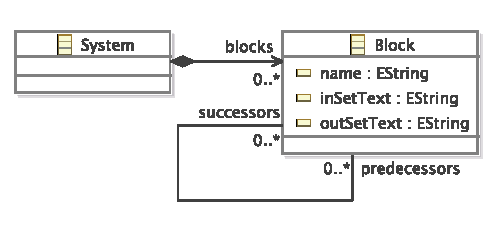
\includegraphics[scale=0.75]{4.Analysis/fptc_before.pdf}
  \caption{Original metamodel, prior to evolution.}
  \label{fig:mm_before}
\end{figure}

Further analysis of the domain revealed that extra information about the relationship between \texttt{Block}s needed to be stored. The evolved metamodel is shown in Figure~\ref{fig:mm_after}. The \texttt{Connection} class is introduced to capture this extra information. \texttt{Block}s are no longer related directly to \texttt{Block}s, instead they are related via an instance of the \texttt{Connection} class. The \texttt{incomingConnections} and \texttt{outgoingConnections} references of \texttt{Block} are used to relate \texttt{Block}s to each other via an instance of \texttt{Connection}.

\begin{figure}[htbp]
  \centering
  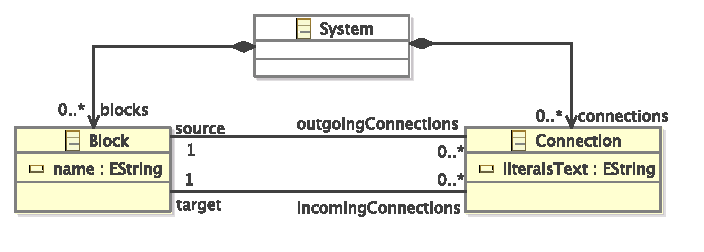
\includegraphics[scale=0.75]{4.Analysis/fptc_after.pdf}
  \caption{Evolved metamodel with Connection metaclass.}
  \label{fig:mm_after}
\end{figure}

A model that conforms to the original metamodel (Figure~\ref{fig:mm_before}) might not be conform to the evolved metamodel (Figure~\ref{fig:mm_after}). Below is a description of the strategy used by the Epsilon FPTC tool to migrate a model from original to evolved metamodel:

\begin{enumerate}
	\item For every instance, \texttt{b}, of \texttt{Block}:
		\subitem For every successor, \texttt{s}, of \texttt{b}:
			\subsubitem Create a new instance, \texttt{c}, of \texttt{Connection}.
			\subsubitem Set \texttt{b} as the \texttt{source} of \texttt{c}.
			\subsubitem Set \texttt{s} as the \texttt{target} of \texttt{c}.
			\subsubitem Add \texttt{c} to the \texttt{connections} reference of the \texttt{System} containing \texttt{b}.
	\item And nothing else changes.
\end{enumerate}


Differencing and change recording metamodel matching approaches are now compared and contrasted. 

\paragraph{Change recording}
In change recording approaches, metamodel evolution is monitored by a tool, which records a list of primitive changes (e.g. Add class named \texttt{Connection}, or Change the type of feature \texttt{successors} from \texttt{Block} to \texttt{Connection}). The record of changes may be reduced to a normal form, which might remove redundancy, but might also erase useful information. In change recording, some types of metamodel evolution can be more easily recognised than with differencing. With change recording, renaming of a metamodel element from X to Y can be distinguished from the following sequence: remove a metamodel element called X, add a metamodel element called Y. With differencing, this distinction is not possible.

In general, more than one combination of primitive changes can be used to achieve the same metamodel evolution. However, when recording changes, the way in which a metamodel is evolved affects the inference of migration strategy. In the example presented above, the \texttt{outgoingConnections} reference (shown in Figure~\ref{fig:mm_after}) could have been produced by changing the name and type of the \texttt{successors} reference (shown in Figure~\ref{fig:mm_before}). In this case, the record of changes would indicate that the new \texttt{outgoingConnections} reference is an evolution of the \texttt{successors} reference, and consequently inferred migration strategy would likely migrate values of \texttt{successors} to values of \texttt{out\-go\-ingCon\-nect\-ions}. Alternatively, the metamodel developer may have elected to delete the \texttt{successors} reference and then create the \texttt{out\-go\-ingCon\-nect\-ions} reference afresh. In this record of changes, it is less obvious that the migration strategy should attempt to migrate values of \texttt{successors} to values of \texttt{out\-go\-ingCon\-nect\-ions}. Change recording approaches require the metamodel developer to consider the way in which their metamodel changes will be interpreted.

Change recording approaches require facilities for monitoring metamodel changes from the metamodel editing tool, and from the underlying modelling framework. As with operation-based co-evolution, it is not clear to what extent change recording can be supported when a textual syntax is used to evolve a metamodel. A further challenge is that the granularity of the metamodel changes that can be monitored influences the inference of the migration strategy, but this granularity is likely to be controlled by the modelling framework.


\paragraph{Differencing}
In differencing approaches, the original and evolved metamodels are compared to produce the difference model. Unlike change recording, metamodel evolution may be performed using any metamodel editor; there is no need to monitor the primitive changes made to perform the metamodel evolution. However, as discussed above, not recording the primitive changes can cause some categories of change to become indistinguishable, such as renaming versus a deletion followed by an addition.

To illustrate this problem further, consider again the metamodel evolution described above. A comparison of the original (Figure~\ref{fig:mm_before}) and evolved (Figure~\ref{fig:mm_after}) metamodels shows that the references named \texttt{successors} and \texttt{predecessors} no longer exist on \texttt{Block}. However, two other references, named \texttt{out\-go\-ingCon\-nect\-ions} and \texttt{incomingConnections}, are now present on \texttt{Block}. A metamodel matching approach might deduce (correctly, in this case) that the two new references are evolutions of the old references. However, no metamodel matching approach is able to determine which mapping is correct from the following two possibilities:

\begin{itemize}
	\item \texttt{successors} evolved to \texttt{incomingConnections}, and \texttt{predecessors} evolved to \texttt{outgoingConnections}.
	\item \texttt{successors} evolved to \texttt{outgoingConnections}, and \texttt{predecessors} evolved to \texttt{incomingConnections}.
\end{itemize}

The choice between these two possibilities can only made by the metamodel developer, who knows that \texttt{successors} (\texttt{predecessors}) is semantically equivalent to \texttt{outgoingConnections} (\texttt{incomingConnections}). As shown by this example, fully automatic differencing approaches cannot always infer a migration strategy that will capture the semantics desired by the metamodel developer.


\subsection{Summary}


\section{Requirements Identification}
\label{sec:requirements_identification}
% The analysis of existing techniques will lead to requirements for our research. We will conclude the chapter by enumerating these requirements, refining the high-level research objectives from the literature review chapter into lower-level research objectives.


When a metamodel change will affect conformance in only a small number of models, a metamodel developer may decide that the extra effort required to specify an executable migration strategy is too great, and prefer a user-driven co-evolution approach. Because no existing work has explored user-driven co-evolution and several of the co-evolution examples identified in Section X used a user-driven co-evolution approach, part of this thesis concentrated on exploring user-driven co-evolution.

% Summarise the charactersitics of modelling frameworks that restrict the management of co-evolution. Link to section of implementation that will address these restrictions.


% Summarise problems with developer-driven co-evolution approaches, leading to requirements that can later be refined into a need for a domain-specific language for migration (e.g. capturing patterns, providing a language for presenting alternative migration strategies, providing a language for clearly communicating the effects of migration to aid in the selection of a co-evolution operator, reduce the amount of effort required to specify migration etc)

